\chapter{Implementation}



\section{Javascript Cryptography}

\paragraph{Originally, the researcher was not sure how best to implement cryptography within a Thunderbird add-on. Implementing my own javascript AES algorithm, while ideal, was not realistic--or adviceable--with the time constraints of this thesis. Thus, the issue would be finding an existing library or API that had done the javascript cryptographic implementations.}

\paragraph{For this task, there were three necessary conditions:}

\begin{itemize}
\item A clear, easily identifiable, and reputable source/owners
\item Existing, easily obtainable, and comprehensive documentation
\item Open source, easily available code
\end{itemize}

\paragraph{and, slightly less important, actively maintained.}

\paragraph{Meeting the above criteria was not as simple as it would seem. There were many options that met some of the conditions, but meeting them all was more challenging. Ultimately, however, the researcher was satisfied with the Stanford Javascript Crypto Library (SJCL) meeting the above full criteria.}\cite[Website]{SJCL}

\paragraph{The usage is pretty straight forward, and will work for this implementation. Simply linking the javascript source in the html file (See reference figure: \ref{fig: exampleSJCL_html}).:}

\begin{figure}[H]
\begin{minted}[breaklines]{html}
<!DOCTYPE html>
<html>
<head>
    <meta charset="utf-8"/>
    <script src="http://bitwiseshiftleft.github.io/sjcl/sjcl.js"></script>
</head>
</html>
\end{minted}
\caption{\label{fig: exampleSJCL_html} Example of linking SJCL in HTML}
\end{figure}

\paragraph{and, the javascript can simply be used as follows (See reference figure: \ref{fig: exampleSJCL_js}):}

\begin{figure}[H]
\centering
\begin{minted}[breaklines]{javascript}
var ciphertext = sjcl.encrypt("reallyHardPasswordNoOneCouldEveryGuess", "Hello World!");
var plaintext = sjcl.decrypt("reallyHardPasswordNoOneCouldEveryGuess", ciphertext);
console.log("plain text: " + plaintext);
console.log("cipher text: " + ciphertext);
console.log("plain text - again!: " + plaintext);
\end{minted}
\caption{\label{fig: exampleSJCL_js} Example of javascript SJCL}
\end{figure}

\paragraph{giving the following result (See reference figure: \ref{fig: exampleSJCL}):}

\begin{figure}[H]
\centering
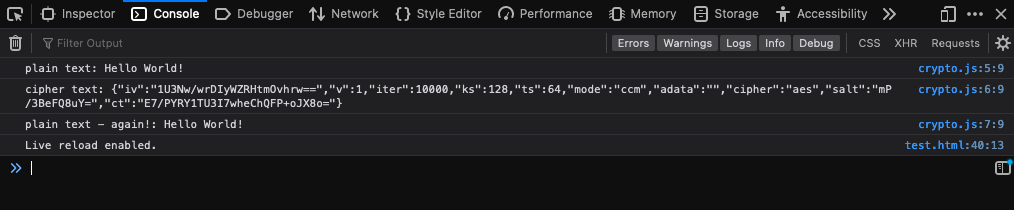
\includegraphics[width=0.9\textwidth]{exampleSJCL.png}
\caption{\label{fig: exampleSJCL} Example output to Firefox console}
\end{figure}

\paragraph{The usage is pretty straight forward, and will meet our needs.}

\section{WebExtensions}

\paragraph{WebExtensions are web technology built with typical Web elements such as HTML, CSS, and javascript. Each extension must also have a \emph{manifest.json} file which carries vital information about the extension. This may include properties--known as manifest keys--like the author of the software extension, software version, permissions, and/or minimum requirement of Thunderbird to use the extension, just to name a few. As the author delves into the development section, it will be pretty clear how they work.} \cite[Webpage]{WebEx}

\paragraph{Starting with the release of Thunderbird version 68 (August 2019), Thunderbird moved to only support WebExtensions for add-ons and themes development, with all previous versions no longer working.}

\paragraph{Here is an image from Mozilla's Thunderbird Add-on Webpage that gives a quick glance of how the extensions might look like.}\footnote{Source: same webpage as noted above.}


\begin{figure}[H]
\centering
\includegraphics[width=0.9\textwidth]{webEx.png}
\caption{\label{fig: webEx} WebExtension overview}
\end{figure}


\section{Implementation Details}

